\newcommand{\pitwo}{\frac{\pi}{2}}
\newcommand{\newpar}{\vspace{1em}\noindent}

\chapter{Funktionen}
\label{chap:funktionen}

Autor: Gerhard Gossen

\mbox{}\par
%\section{Definition}
\noindent Eine Funktion $f$ ist eine Abbildung, die einem Wert aus dem \emph{Definitionsbereich $D(f)$} genau einen Wert aus dem \emph{Wertebereich $W(f)$} zuordnet. Die übliche Darstellung ist
$f : X \to Y$ (sprich: $f$ ist eine Abbildung von $X$ nach $Y$), wobei $X$ die Definitionsmenge ($D(f) \subseteq X$) und $Y$ die Zielmenge ist ($W(f) \subseteq Y$). Definitions- und Zielmenge sind oft $\R$ (die reellen Zahlen).

\noindent Verbreitete Funktionen sind z.B. Geraden ($f(x) = m\cdot x +n$), Polynome ($f(x) = a_n x^n + a_{n-1} x^{n-1}+\dots + a_1x+a_0$), die trigonometrischen Funktionen ($\sin x$, $\cos x$, $\tan x$, siehe Abschnitt~\ref{sec:trigonometrie}) oder Exponentialfunktionen ($a^x$, siehe Abschnitt~\ref{sec:exponential}). Abbildung~\ref{fig:Funktionssammlung} zeigt die Graphen einiger Funktionen.

\begin{figure}[bth]
\begin{center}
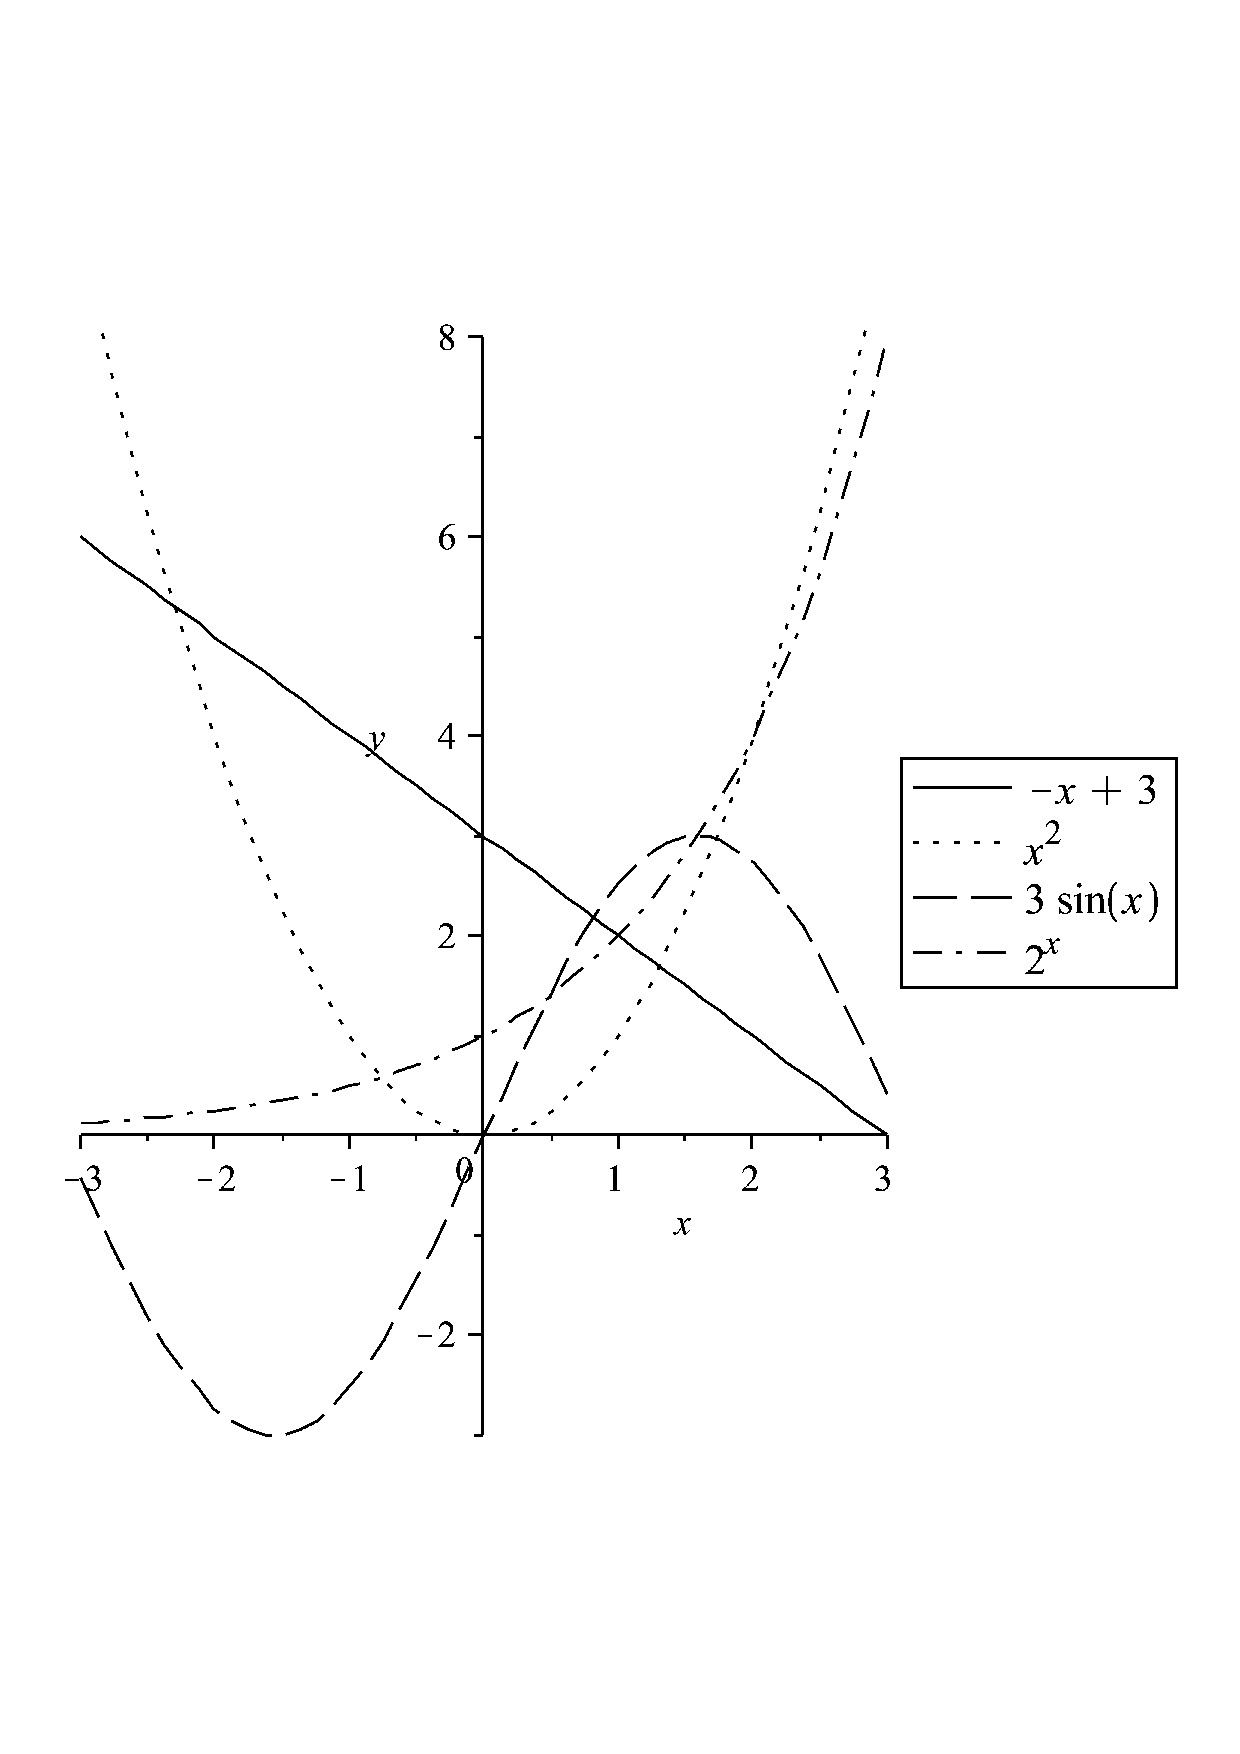
\includegraphics[width=.4\textwidth]{img/Funktionssammlung.pdf}
\end{center}
\caption{Bekannte Funktionen}
\label{fig:funktionen}
\end{figure} 

\noindent Alle Funktionen, die wir im Vorkurs behandeln, sind Funktionen mit \emph{einer Ver"-änderlichen}, also Funktionen, die von einer einzigen Variable (meist $x$) ab"-hän"-gen.Die Eigenschaften einer Funktion kann man über eine \emph{Kurvendiskussion} (siehe Abschnitt~\ref{sec:kurvendiskussion}) herausbekommen. Zuerst werden wir aber zwei wichtige Funktionsfamilien vorstellen: die trigonometrischen Funktionen (Winkelfunktionen, Abschnitt~\ref{sec:trigonometrie}) und die Exponentialfunktionen (Abschnitt~\ref{sec:exponential}).

%%%%%%%%%%%%%%%%%%%%%%%%%%%%%%%%%%%%%%%%%%%%%%%%%%%%%%%%%%%%%%%%%%%%%%%%%%%%%%%%%%%%%%
\section{Trigonometrische Funktionen}
\label{sec:trigonometrie}

Die trigonometrischen Funktionen $\sin, \cos, \tan$ sind die
Winkelfunktionen. Sie sind für Winkel im Bogenmaß definiert (z.\,B. $ x =
\pitwo$). Winkel im Gradmaß (z.\,B. $ x = 90^\circ$) können
eindeutig ins Bogenmaß umgerechnet werden ($90^\circ \equiv \pitwo$).
Deswegen ist auch die Schreibweise $\sin 90^\circ$ möglich.

\subsection{Definition}
Im rechtwinkligen Dreieck gilt:

\begin{minipage}{.5\linewidth}
\begin{eqnarray*}
 \sin x &=& \frac{\text{Gegenkathete}}{\text{Hypothenuse}}\\
 \cos x &=& \frac{\text{Ankathete}}{\text{Hypothenuse}}\\
 \tan x &=& \frac{\text{Gegenkathete}}{\text{Ankathete}} =
\frac{\sin x}{\cos x}
\end{eqnarray*}
\end{minipage}\hspace{.1\linewidth}
\begin{minipage}{.35\textwidth}
 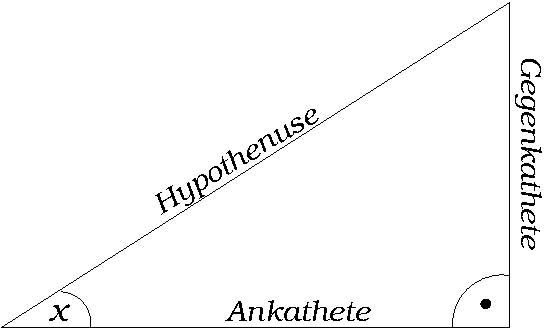
\includegraphics[width=\textwidth]{img/winkel.pdf}
%\vspace{.1em}
\end{minipage}

\noindent Diese Definitionen lassen sich verallgemeinern, so dass die Funktionen für 
alle reelen Zahlen definiert sind (im rechtwinkligen Dreieck:
$0\leq x \leq 90^\circ$). Damit ergeben sich diese Funktionen:
\begin{center}\hfill
\begin{minipage}{.25\textwidth}
 \begin{center}
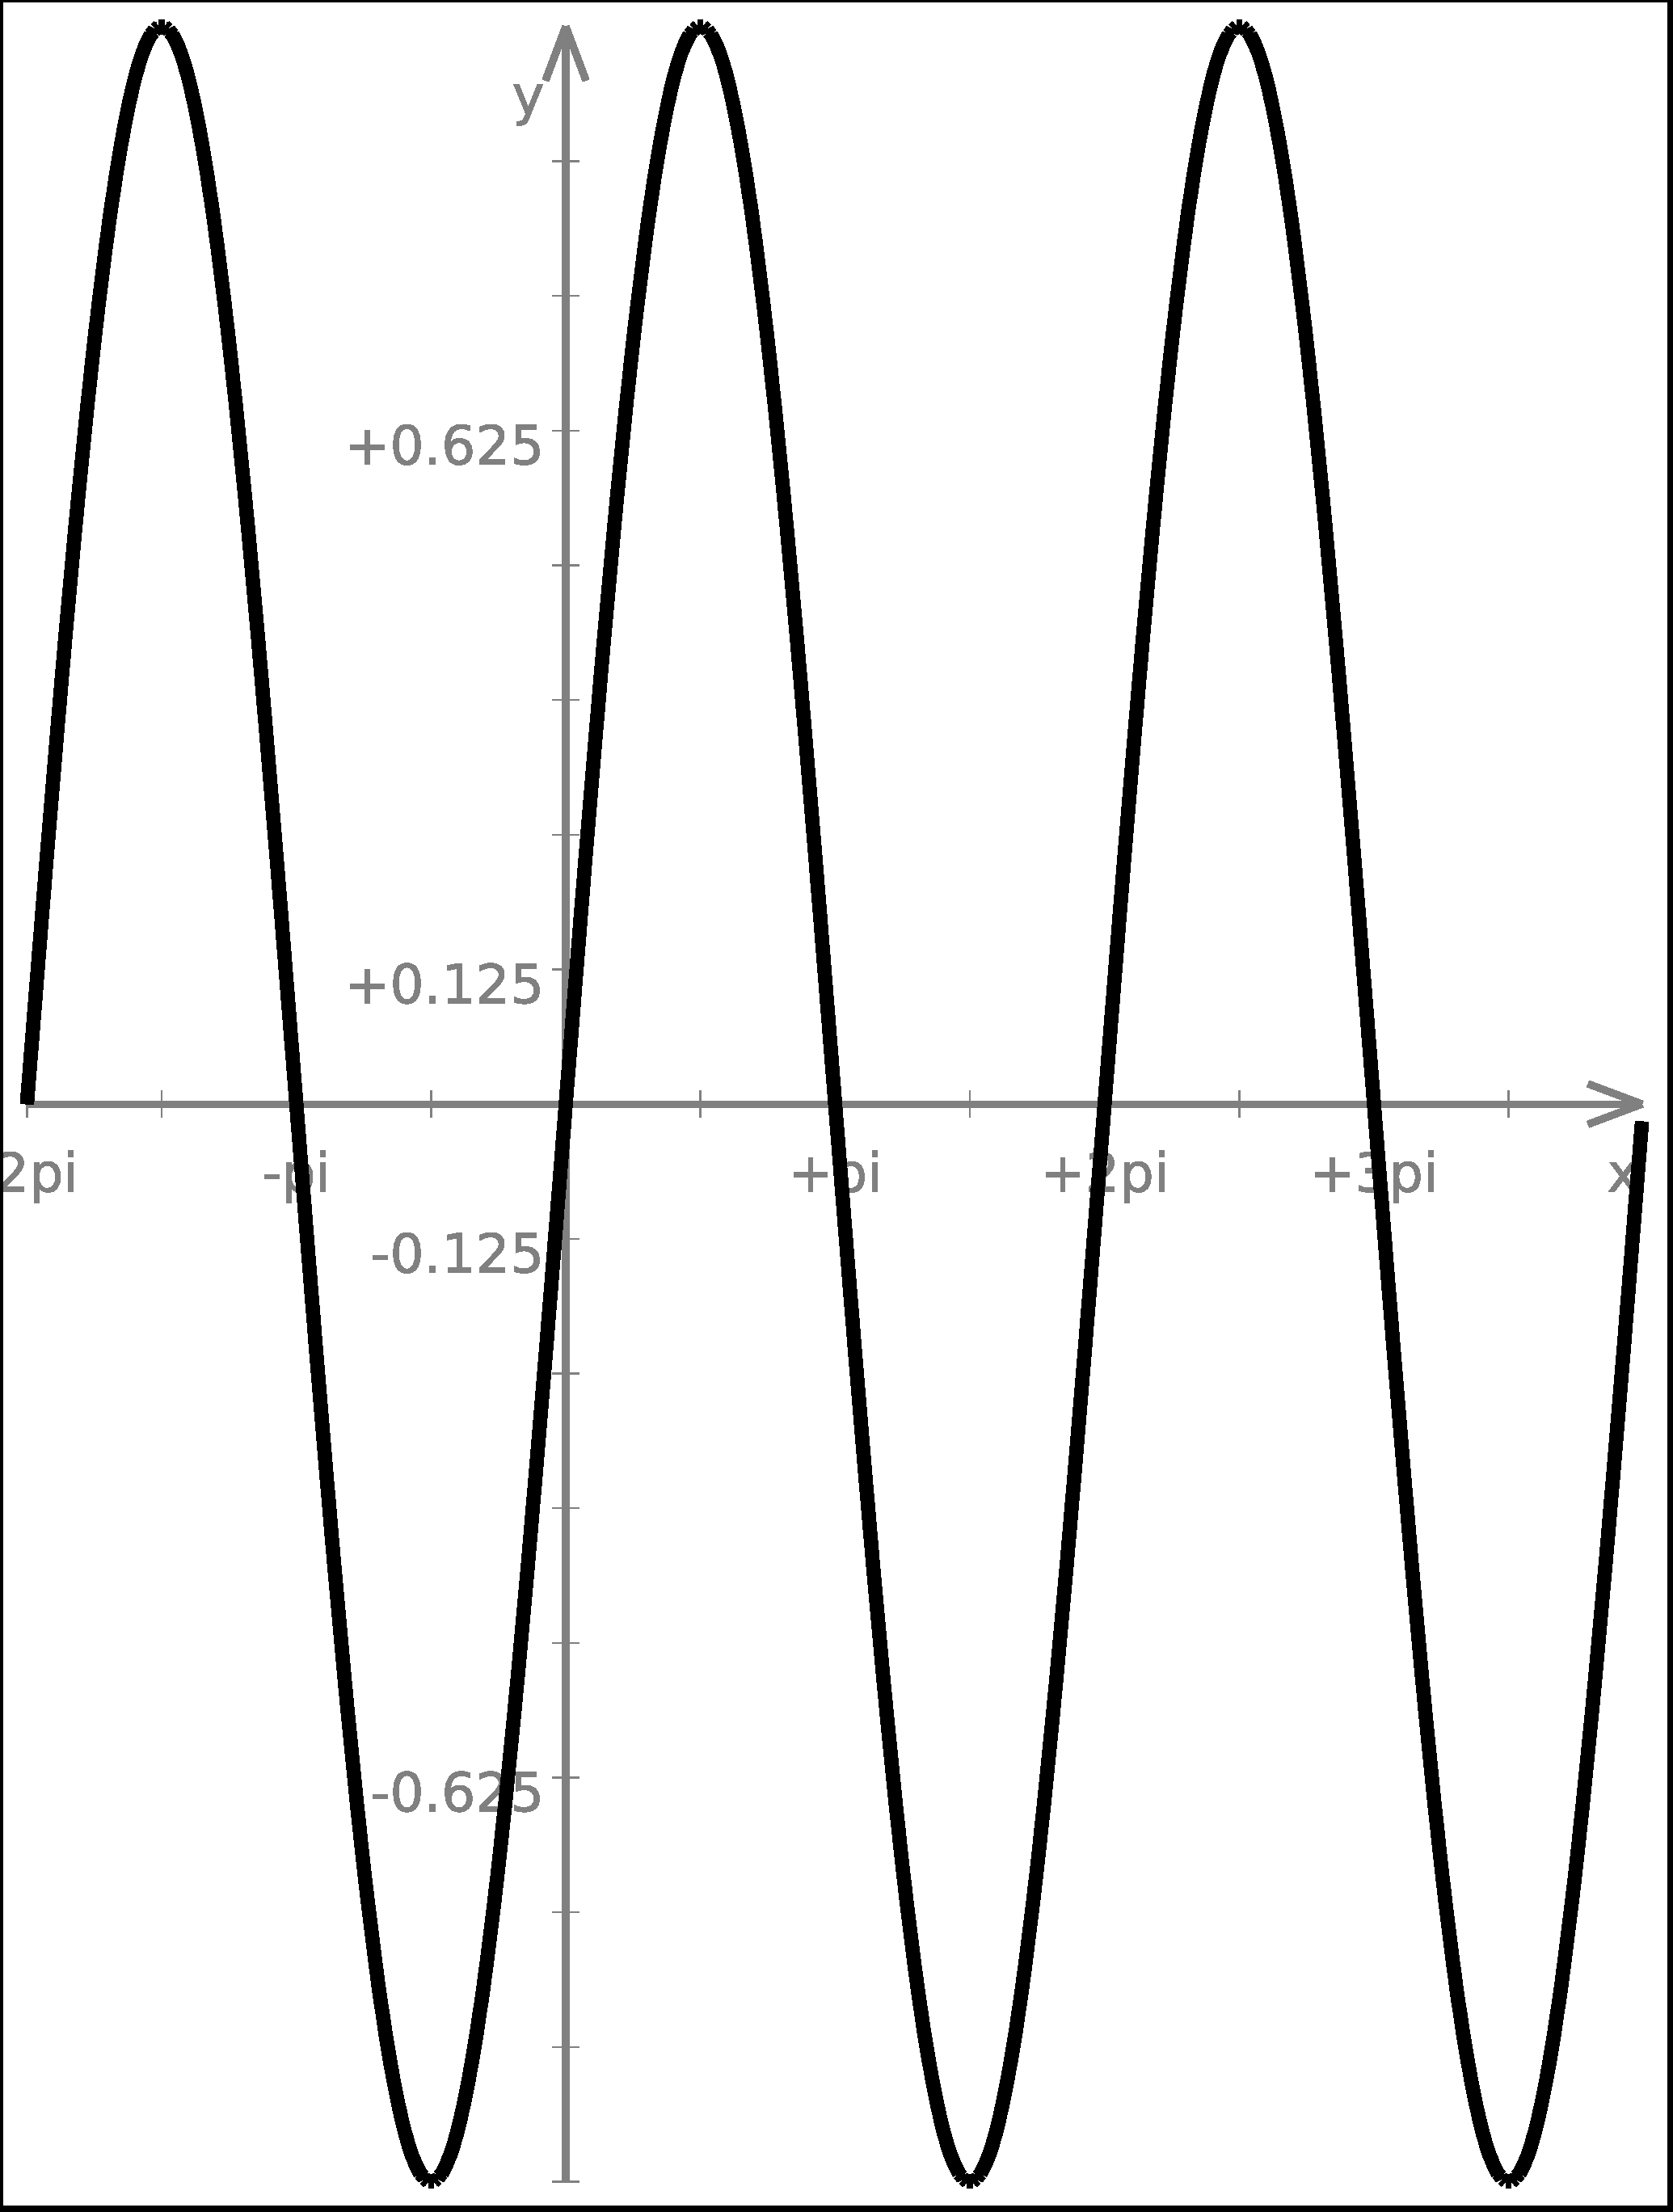
\includegraphics[width=\textwidth, height=2.5cm]{img/sin.pdf}
 $\sin x$         \end{center}
\end{minipage}\hfill
\begin{minipage}{.25\textwidth}
 \begin{center}
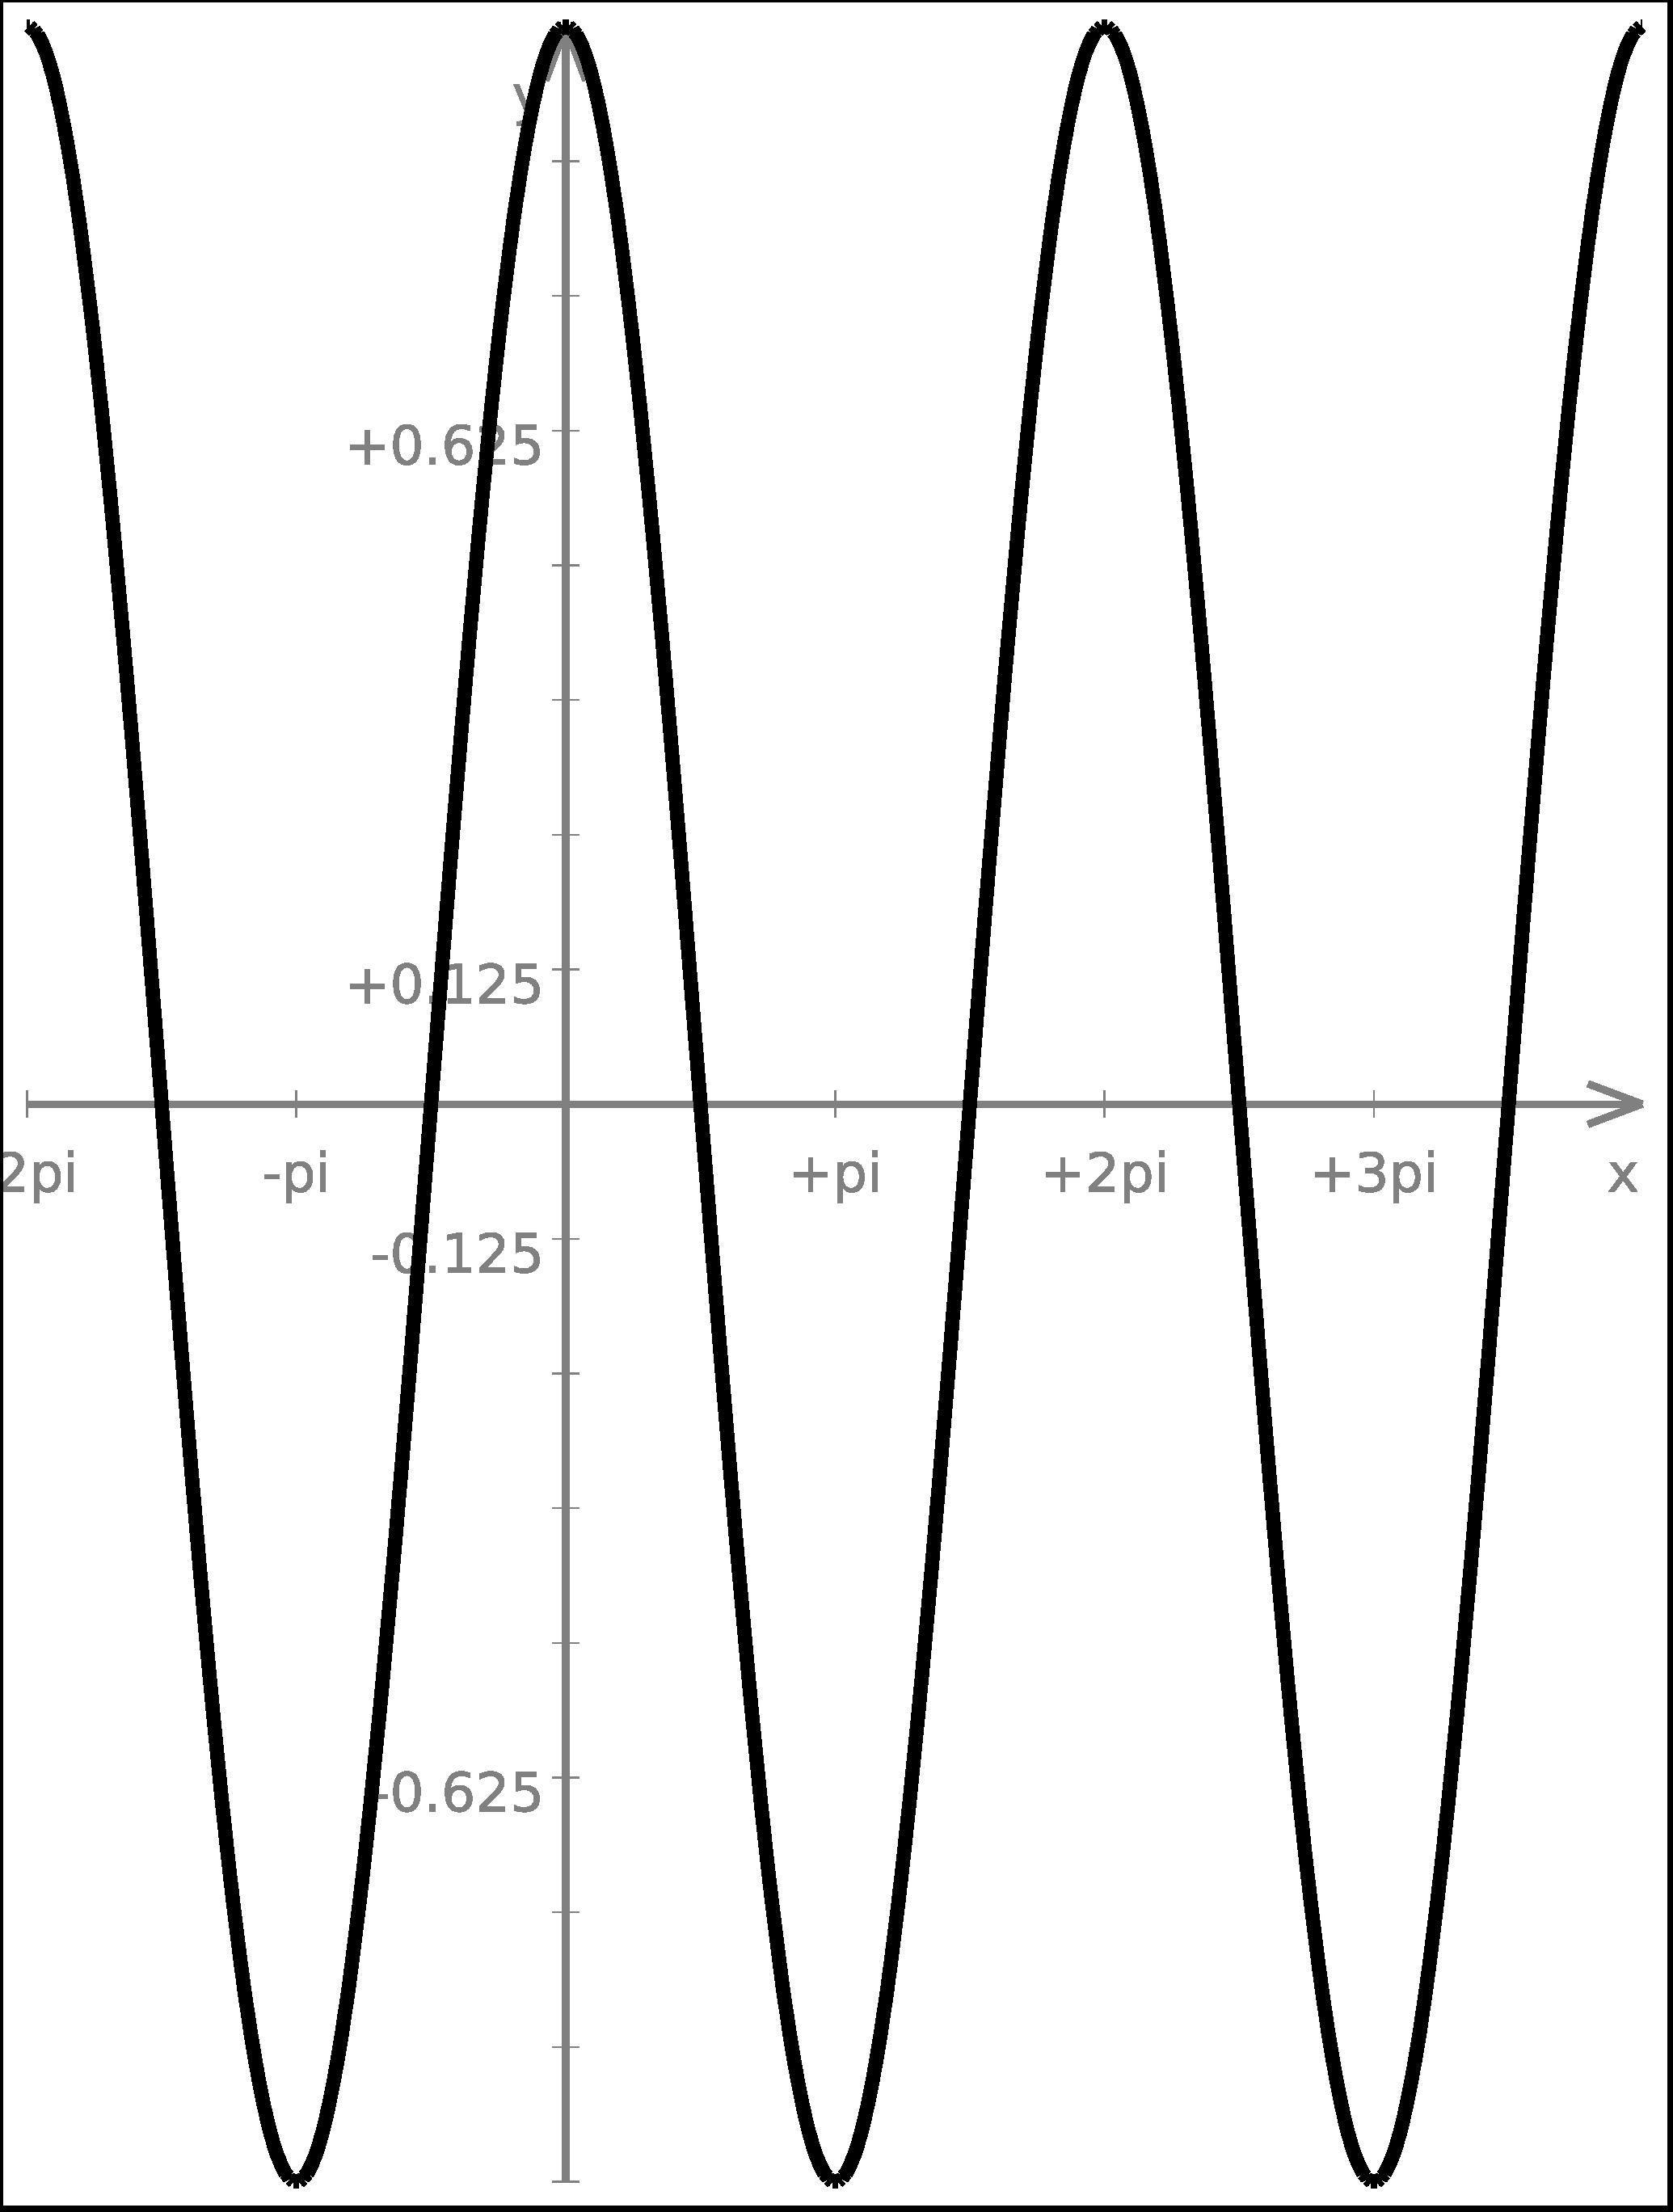
\includegraphics[width=\textwidth, height=2.5cm]{img/cos.pdf}
 $\cos x$ \end{center}
\end{minipage}\hfill
\begin{minipage}{.25\textwidth}
 \begin{center}
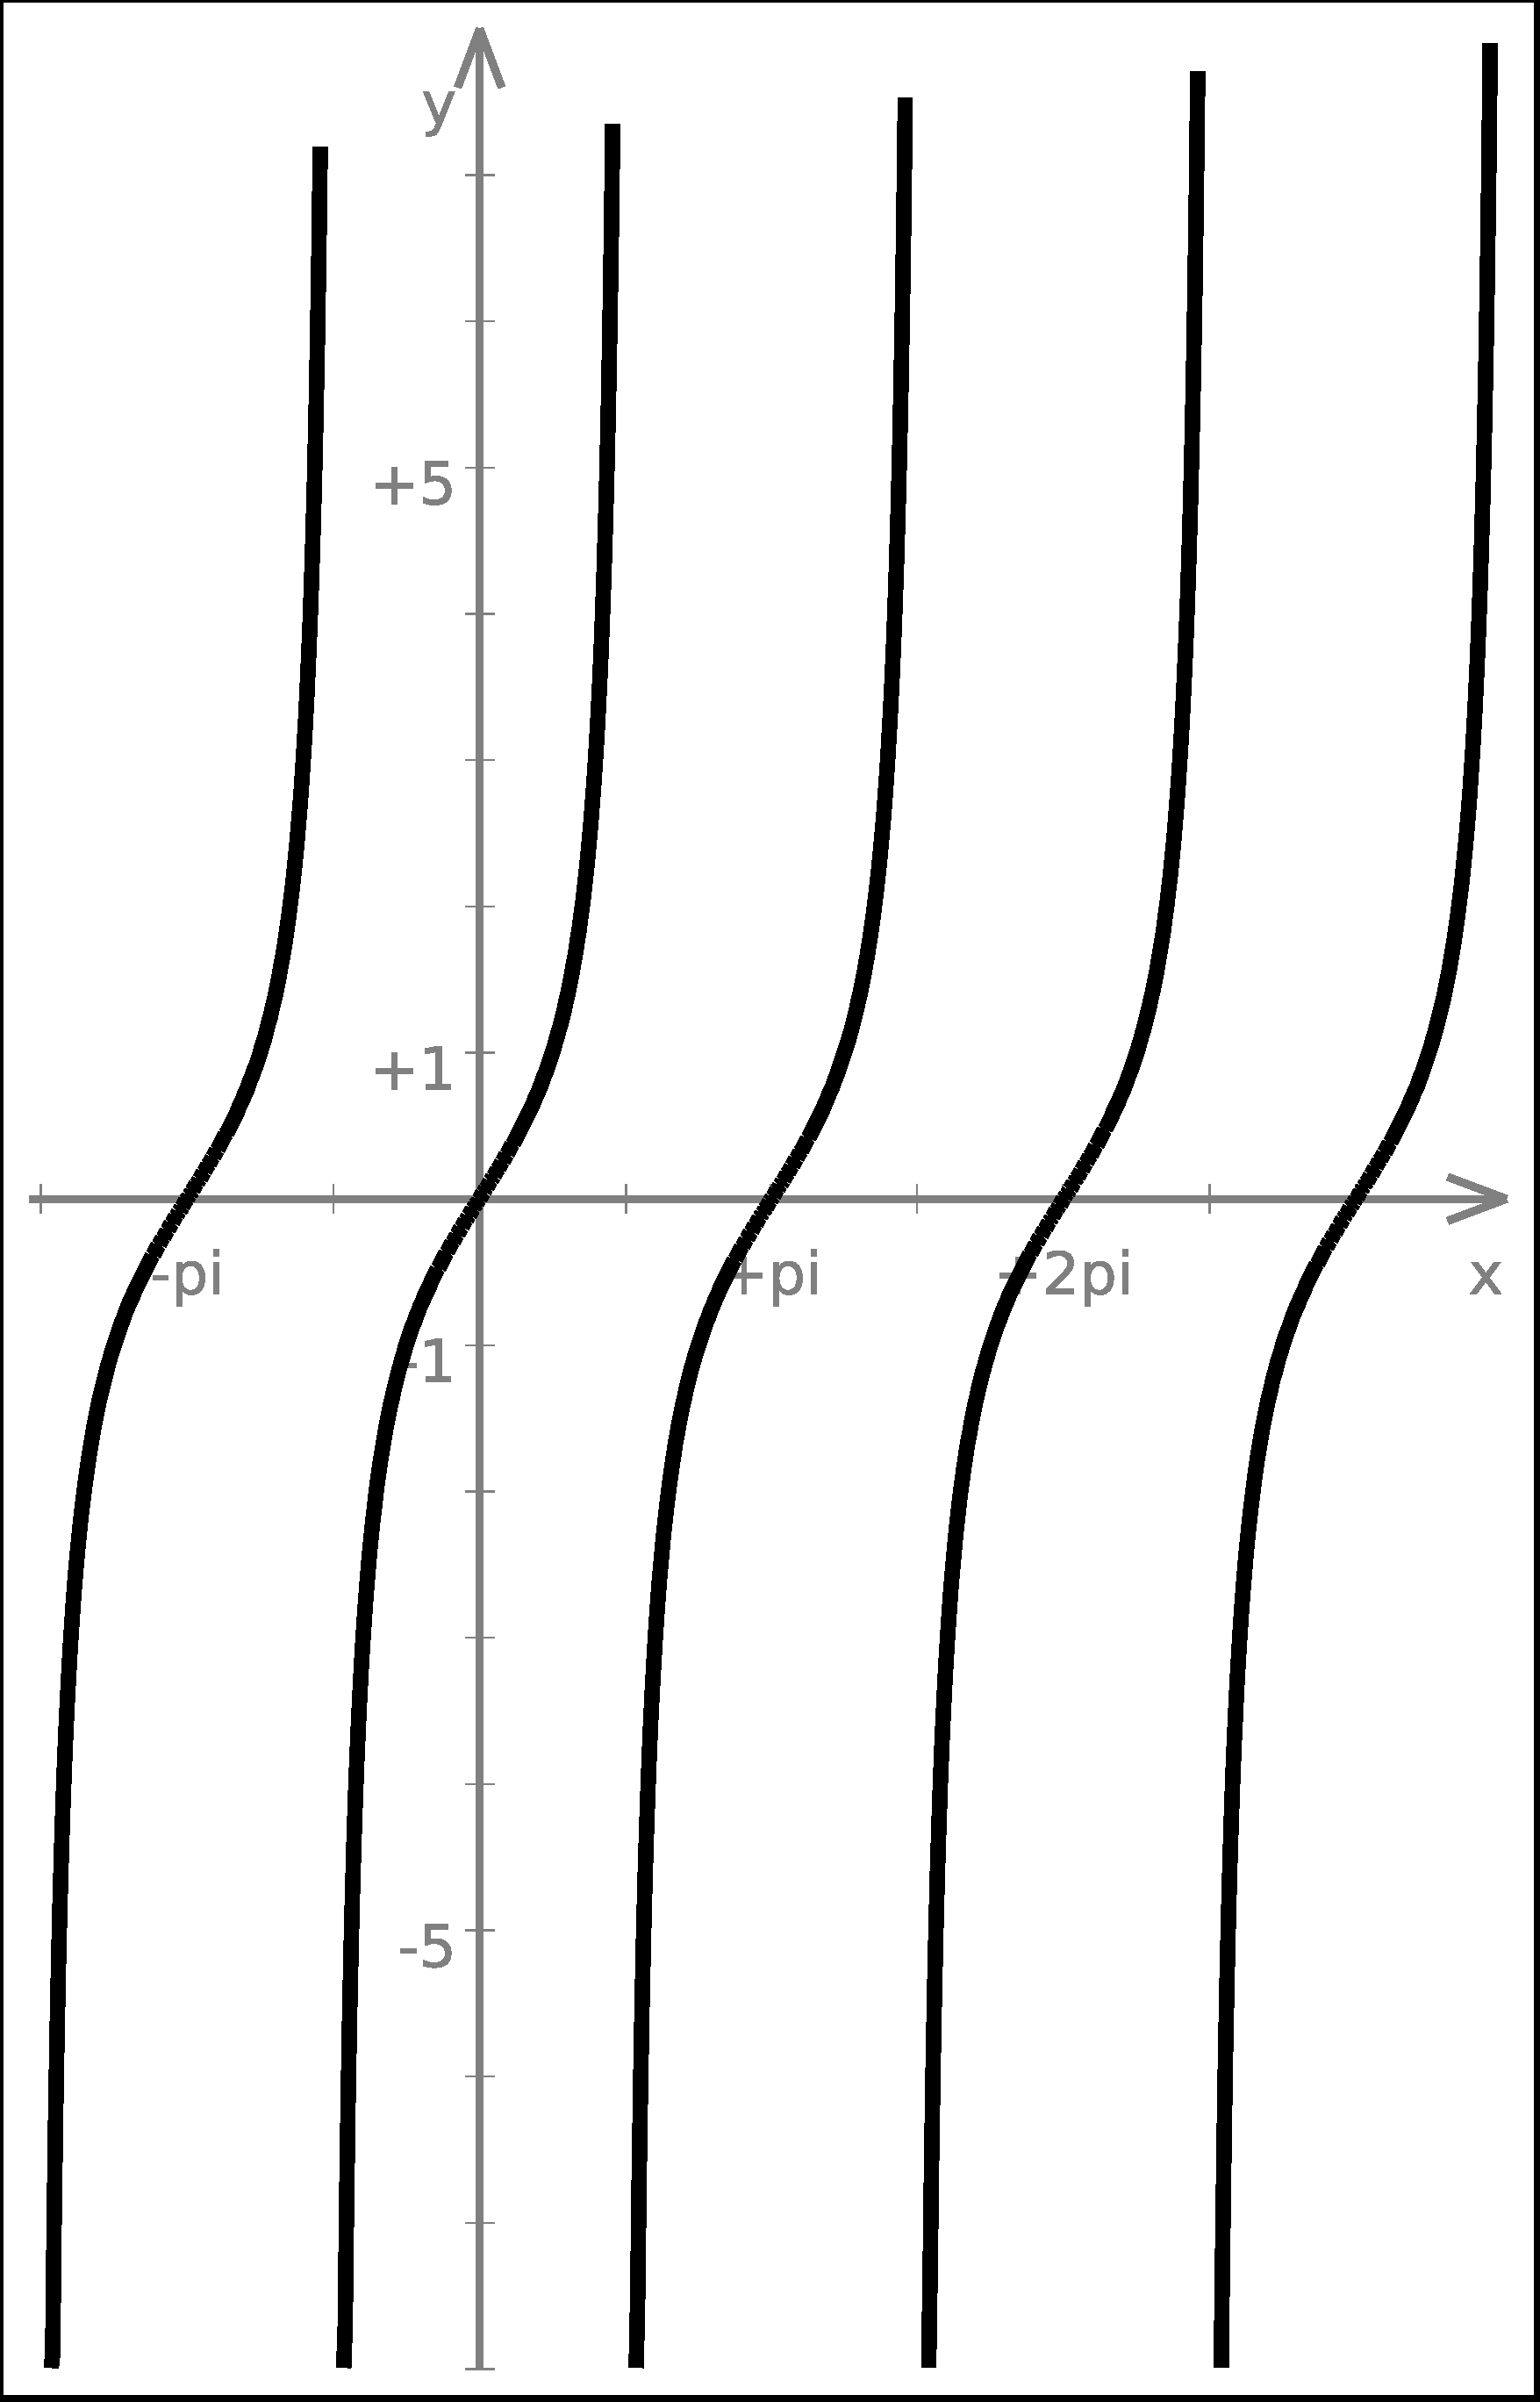
\includegraphics[width=\textwidth, height=4cm]{img/tan.pdf} 
 $\tan x$         \end{center}
\end{minipage}\hfill
%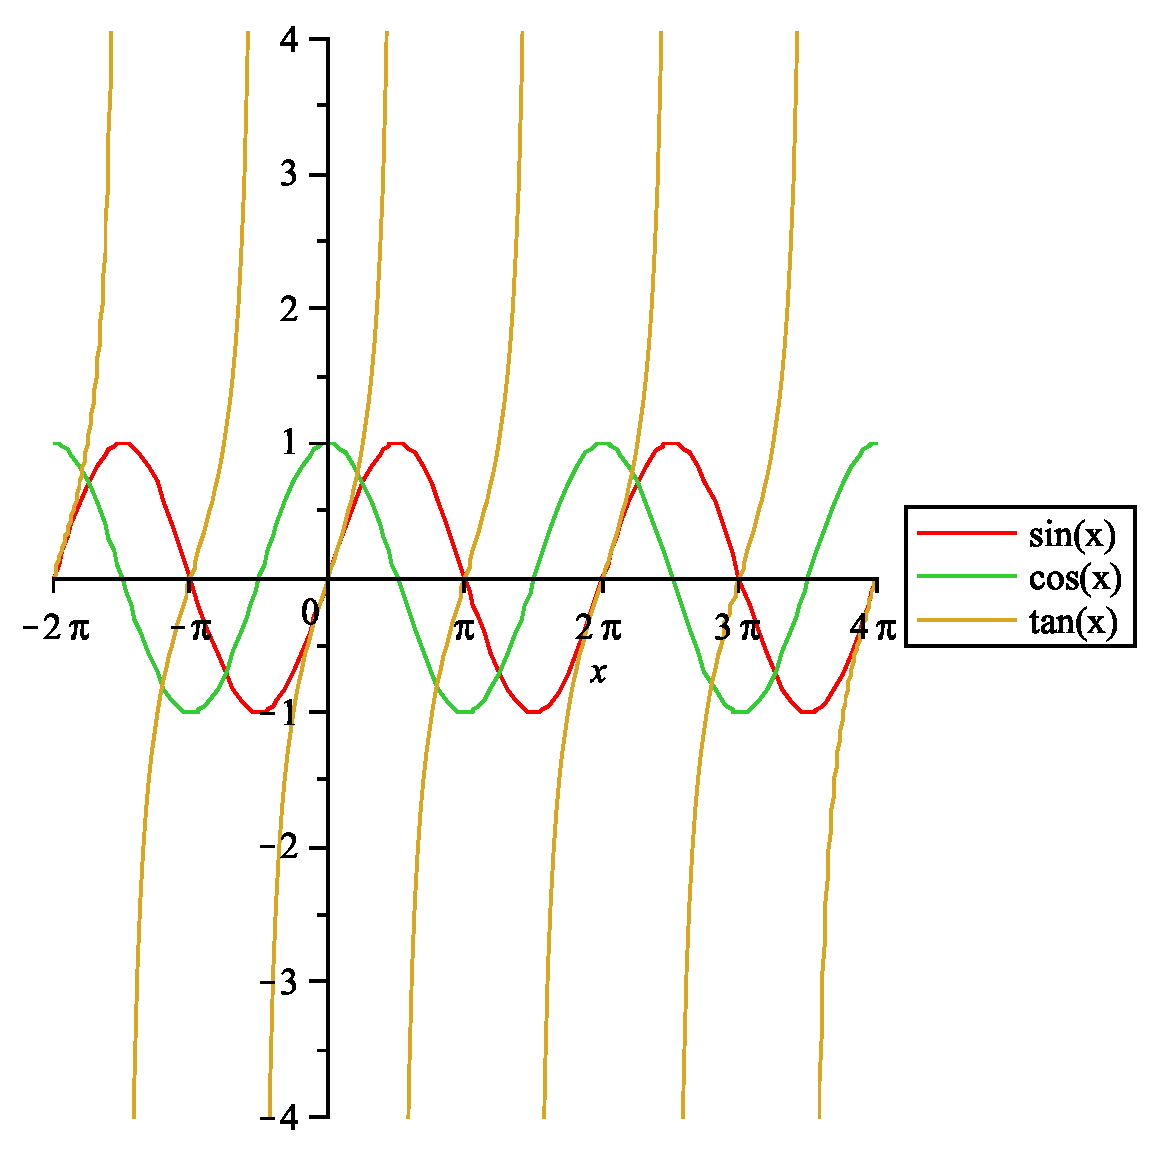
\includegraphics[height=8cm]{img/trig.pdf}
\end{center}

\noindent Man sieht, dass der Cosinus gegenüber dem Sinus nur um $\pitwo$
verschoben ist, es gilt also:
\[\sin \left( \pitwo-x \right) = \cos x \qquad
\cos \left( \pitwo-x\right) = \sin x\]

Beispiel:
\begin{gather*}
\cos\left(\pitwo\right) = \sin\left(\pitwo - \pitwo \right)= \sin(0) = 0\\
\displaybreak[0]
\sin\left(\frac{3\pi}{2} \right) = \cos\left(\pitwo - \frac{3\pi}{2} \right)
= \cos(-\pi) = -1
\end{gather*}

\subsection{Periodizität und Symmetrie}\label{sec:trig:perioden}
Alle Winkelfunktionen sind periodisch, d.~h. alle Werte wiederholen sich in
regelmäßigen Abständen. Es gilt also für jede ganze Zahl $k$:
\[\sin(x+2k\pi) = \sin x \quad \cos(x+2k\pi) = \cos x \quad \tan(x+k\pi) =
\tan x\] (Zur Erinnerung: $2\pi \equiv 360^\circ$, deswegen entspricht $2k\pi$ genau $k$ Vollkreisen).

\newpar
Beispiele:
\begin{gather*}
\sin\left(\pitwo\right) = \sin\left(\frac{5\pi}{2} \right)=
\sin\left(\frac{9\pi}{2} \right)= \sin\left(\frac{13\pi}{2} \right) = \dots\\
\cos(\pi) = \cos(3\pi) = \cos(5\pi) = \cos(7\pi) = \dots\\
\tan\left(\frac{\pi}{4}\right) = \tan\left(\frac{3\pi}{4}\right) =
\tan\left(\frac{5\pi}{4}\right) = \tan\left(\frac{5\pi}{4}\right) = \dots
\end{gather*}

\newpar

\noindent Die Sinus- und Cosinusfunktion sind symmetrisch, der Sinus ist
punktsymmetrisch zum Ursprung, der Cosinus achsensymmetrisch zur $y$-Achse.
Zusammen mit der Periodizität folgen daraus folgende Beziehungen:

\begin{align*}
\text{\scriptsize(2) } \sin(\pi-x)&= \phantom{-}\sin x& \cos(\pi-x)&=-\cos x &
\tan(\pi-x)
&= -\tan x\\
\text{\scriptsize(3) }\sin(\pi+x)&= -\sin x & \cos(\pi+x)&=-\cos x &
\tan(\pi+x)
&= \phantom{-}\tan x\\
\text{\scriptsize(4) } \sin(2\pi-x)&= -\sin x& \cos(2\pi-x)&=\phantom{-}\cos x
& \tan(2\pi-x)
&= -\tan x\\
\end{align*}

\noindent Das Vorzeichen ist also vom Quadranten abhängig, in dem sich $x$ befindet.
Diesen Zusammenhang zeigt Abbildung 7.2.

%\begin{center}
% 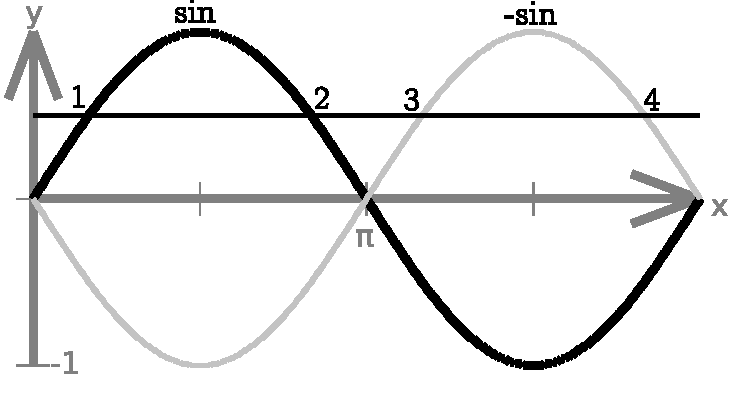
\includegraphics[width=.4\textwidth]{img/sin_sym.pdf}
%\end{center}
\begin{figure}[hbt]
\noindent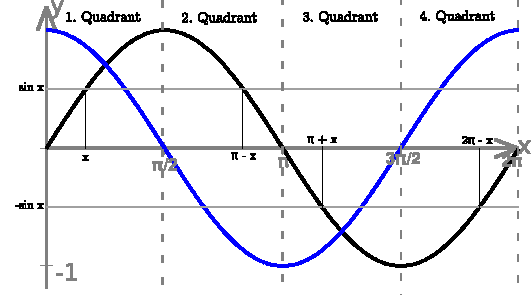
\includegraphics{img/symmetrie.pdf}

\vspace{-.15cm}
\hspace{.68cm}
\begin{tabular}{|p{1.56cm}|p{1.6cm}|p{1.6cm}|p{1.55cm}|}
 $\sin x$ & $+\sin x$ & $-\sin x$ & $-\sin x$\\
 $\cos x$ & $-\cos x$ & $-\cos x$ & $+\cos x$\\
 $\tan x$ & $-\tan x$ & $+\tan x$ & $-\tan x$\\
\hline
\end{tabular}
\label{fig:symmetrie}
\caption{Symmetrie von Sinus und Cosinus}
\end{figure}

\noindent Die Werte für $\sin x, 0 \leq x \leq \pitwo$ reichen damit aus, um alle
Werte für $\sin$ und $\cos$ bestimmen. Die wichtigsten Werte sind in der
folgenden Tabelle.
\[\begin{array}{|r|ccccc|}\hline
 x \text{ im Bogenmaß} & 0 & \frac{\pi}{6} &
\frac{\pi}{4} & \frac{\pi}{3} &
\pitwo\\
 x \text{ im Gradmaß}  & 0 & 30^\circ & 45^\circ & 60^\circ & 90^\circ\\
 \sin x                & \frac{1}{2}\sqrt{0} & \frac{1}{2}\sqrt{1}
& \frac{1}{2}\sqrt{2} &\frac{1}{2}\sqrt{3} & \frac{1}{2}\sqrt{4}\\
 \cos x    & \frac{1}{2}\sqrt{4} & \frac{1}{2}\sqrt{3} & \frac{1}{2}\sqrt{2}
 & \frac{1}{2}\sqrt{1} & \frac{1}{2}\sqrt{0}\\\hline
\end{array}\]



\subsection{Umkehrfunktionen}%: $arcsin$, $arccos$, $arctan$}
Die Umkehrfunktionen zu $\sin$, $\cos$ und $\tan$ sind $\arcsin$, $\arccos$
und $\arctan$ (sprich: \emph{arcus sinus}, \emph{arcus cosinus} und
\emph{arcus tangens}). Da die trigonometrischen Funktionen periodisch sind
(z.~B. gilt $\sin(0) = \sin(2\pi)=0$), kann es keine eindeutige Umkehrfunktion
geben (in diesem Beispiel: ist $\arcsin(0)$ gleich $0$ oder $2\pi$?).
Deswegen sind die Funktionen nur auf einem bestimmten Bereich umkehrbar.
Diese Bereiche sind:
\begin{eqnarray*}
y = \sin x\quad -\pitwo \leq x \leq \pitwo &
\Longleftrightarrow &
x = \arcsin y \quad -1 \leq y \leq 1 \\
y = \cos x\quad \phantom{--}0 \leq x \leq \pi &
\Longleftrightarrow &
x = \arccos y \quad -1 \leq y \leq 1\\
y = \tan x\quad -\pitwo < x < \pitwo &
\Longleftrightarrow &
x = \arctan y \quad y\in \mathbb{R}
\end{eqnarray*}

\subsection{Trigonometrischer Pythagoras}
Für alle $x$ gilt: $\sin^2 x + \cos^2 x = 1$. Diese Aussage heißt auch
\emph{trigonometrischer Pythagoras}. Damit kann manchmal ein Term vereinfacht
werden.

\subsection{Additionstheoreme}
Die Winkelfunktionen haben unter anderem diese wichtigen Eigenschaften:
\begin{eqnarray*}
 \sin(x_1 + x_2) &=& \sin x_1 \cos x_2 + \cos x_1 \sin x_2\\
 \sin(x_1 - x_2) &=& \sin x_1 \cos x_2 - \cos x_1 \sin x_2\\
 \cos(x_1 + x_2) &=& \cos x_1 \cos x_2 - \sin x_1 \sin x_2\\
 \cos(x_1 - x_2) &=& \cos x_1 \cos x_2 + \sin x_1 \sin x_2\\
\end{eqnarray*}

Beispiele:
\begin{align*}
 \sin(120^\circ) &= \sin(60^\circ +60^\circ) =
\sin(\tfrac{\pi}{3}+\tfrac{\pi}{3}) &\text{\scriptsize(wende
Additionstheorem an)}\\\displaybreak[0]
  &= \sin\tfrac{\pi}{3}\cos\tfrac{\pi}{3} +
\cos\tfrac{\pi}{3}\sin\tfrac{\pi}{3}\\
  &= \tfrac{1}{2}\sqrt{3}\cos\tfrac{\pi}{3}
+ \cos\left(\tfrac{\pi}{3}\right)\tfrac{1}{2}\sqrt{3} = \sqrt{3}
\smash{\cos\tfrac{\pi}{3}} &\text{\scriptsize (wandele $\cos$ in $\sin$)}\\
 &= \sqrt{3}\sin\left(\tfrac{\pi}{2} - \tfrac{\pi}{3} \right) =
\sqrt{3}\sin\tfrac{\pi}{6}\\
 &= \tfrac{1}{2}\sqrt{3}
\end{align*}
Probe über Symmetrie:
\begin{align*}
\sin(120^\circ) &= \sin\left(\tfrac{2\pi}{3} \right)
    = \sin(\pi-\tfrac{\pi}{3}) \quad\text{\scriptsize (mit
\ref{sec:trig:perioden}(2)) } \\
  &= \sin(\tfrac{\pi}{3})= \tfrac{1}{2}\sqrt{3}
\end{align*}

\subsection{Aufgaben}

\begin{enumerate}
 \item Berechne mit Hilfe der Tabelle in Abschnitt~\ref{sec:trig:perioden}
folgende Werte:
 \begin{multicols}{4}
  \begin{enumerate}
   \item $\sin \frac{2\pi}{3}$ 
   \item $\sin \frac{5\pi}{6}$
   \item $\sin \pi$
   \item $\sin \frac{3\pi}{2}$
   \item $\sin \frac{11\pi}{6}$
   \item $\sin \frac{7\pi}{3}$
   \item $\sin \frac{29\pi}{6}$
   \item $\sin -\frac{3\pi}{4}$
   \item $\cos \frac{\pi}{6}$
   \item $\cos \frac{\pi}{4}$
   \item $\cos \frac{\pi}{3}$
   \item $\cos \frac{\pi}{2}$
   \item $\cos \frac{11\pi}{6}$
   \item $\cos \frac{3\pi}{4}$
   \item $\cos \frac{2\pi}{3}$
   \item $\cos \frac{4\pi}{6}$
   \item $\cos \frac{7\pi}{3}$
   \item $\cos -\frac{11\pi}{4}$
   \item $\tan \frac{\pi}{6}$
   \item $\tan -\frac{\pi}{3}$
  \end{enumerate}
 \end{multicols}

\item Berechne die fehlenden Seitenlängen. Die
Bezeichnungen entsprechen der nebenstehenden Zeichnung.

\begin{minipage}{6cm}
\begin{tabular}{|ccccc|}
$\alpha$ & $\beta$ & $a$ & $b$ & $c$\\
\hline
& &  & $1$ & $\sqrt{2}$\\
& & 2 &  & 4\\ % b = $\sqrt{12}$
& & $\frac{1}{2}\sqrt{3}$& & $\frac{1}{2}$\\
& & 4 & 3 & \\
$\frac{\pi}{6}$ & & 1 & &\\
&$\frac{\pi}{3}$ & & 2 &\\
\end{tabular}
\end{minipage}
\begin{minipage}{4cm}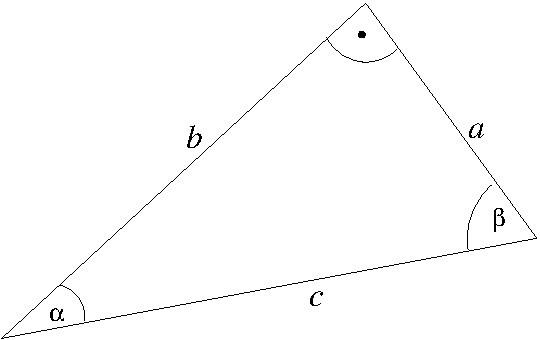
\includegraphics[width=4cm]{img/winkel_aufgaben.pdf}
\end{minipage}




 \item Leite folgende Aussage her: \[ \sin(4\alpha) = 4(\sin\alpha
\cdot \cos^3\alpha - \sin^3\alpha\cdot \cos\alpha)\]
 \item Leite her, dass folgende Aussage gilt:
\[\cos(2\alpha) = 2\cdot\cos^2\alpha -1 \]
 \item* Eine Kugel mit dem Radius 1 umschließt einen Würfel. Bestimme die
maximale Seitenlänge des Würfels.
\end{enumerate}

%%%weiter siehe log_e.tex
